\section{Experiments}
To evaluate BOX, we compare against four other solution-constraint 
-library-based algorithms in various
challenging domains. The first one is random sampling, 
where we uniform sample 
$k$ number of solution constraints. The second one is a 
regular-DOO, which uses Euclidean distance metric to estimate the upper bound
of the constraints, instead of the correlation, the  eqn (\ref{eqn:bc}). This algorithm is 
much motivated by \cite{MunosNIPS11}, which was originally invented for
black box function optimization problems. The third one is static ordering algorithm,
 which orders the grasps according only their
expected values (i.e. eqn (\ref{eqn:b}) without $B_c$)
The last algorithm is Solver - this is what you would do 
if you did not have any of these library-based algorithms to solve the planning problem.
We use RRT seeded with a fixed randomization seed value as our motion 
planner throughout experiments.

To evaluate the speed and quality of plans of these algorithms,
we consider three different plots. 
In the first plot, we primarily compare 
the planning speed of these algorithms by looking at how fast
these algorithms produce the first feasible plan.
In the second plot, we look at, given different
multiples of the time required by Solver to generate
a plan, how much improvements in quality of plans that these
library-based algorithms can provide. Lastly, we look at 
how long these algorithms to take to find the best solution
constraint for the given planning problem instance.

To produce these plots, we run Leave One Out Cross Validation (LOOCV) on the
training data. That is, we assume that we have $n-1$ training problem instances,
and the one that is left out is used as a test problem instance. This is
repeated for all training instances, and the average of $n$ different LOOCV
results are reported.

\subsection{Grasp selection for robust motion planning}
% general description of the task
	% define the task, and what SG represent
In this experiment, the robot needs to plan its left hand motion 
from its initial pose to a pregrasp pose. 
To do this, the robot first needs to
choose a grasp, perform inverse kinemactics to compute the
pregrasp configuration, and then call a motion planner to
compute a path. We would like to choose a grasp such that
the planner, when constraint to plan to the given
pregrasp pose, maximizes the distances to the obstacles
along its trajectory. Therefore, here, our solution constraints
are various grasps. 

% What is a planning problem instnace? how is it generated?
% What's the robot's setup? DOF?
A planning problem instance for
this domain is defined by an arrangement of the 
objects on a table. Figure \ref{fig:grasp_domain}
shows two instances of this problem, which are
also part of the training data. We have four different obstacles
including two mugs, two boxes, and the object to be picked up (the blue object). 
To generate a planning problem instance, we either 
remove an object with probability 0.5, or randomly change
its location on the table. The blue object can only be moved.
The robot's active degrees of freedom (DOF) are its left arm and torso, summing up
to 8 degrees of freedom. Other DOFs remain fixed. The 
robot's initial configuration remains fixed across different 
problem instances as well. 

\begin{figure}[htb]
\centering
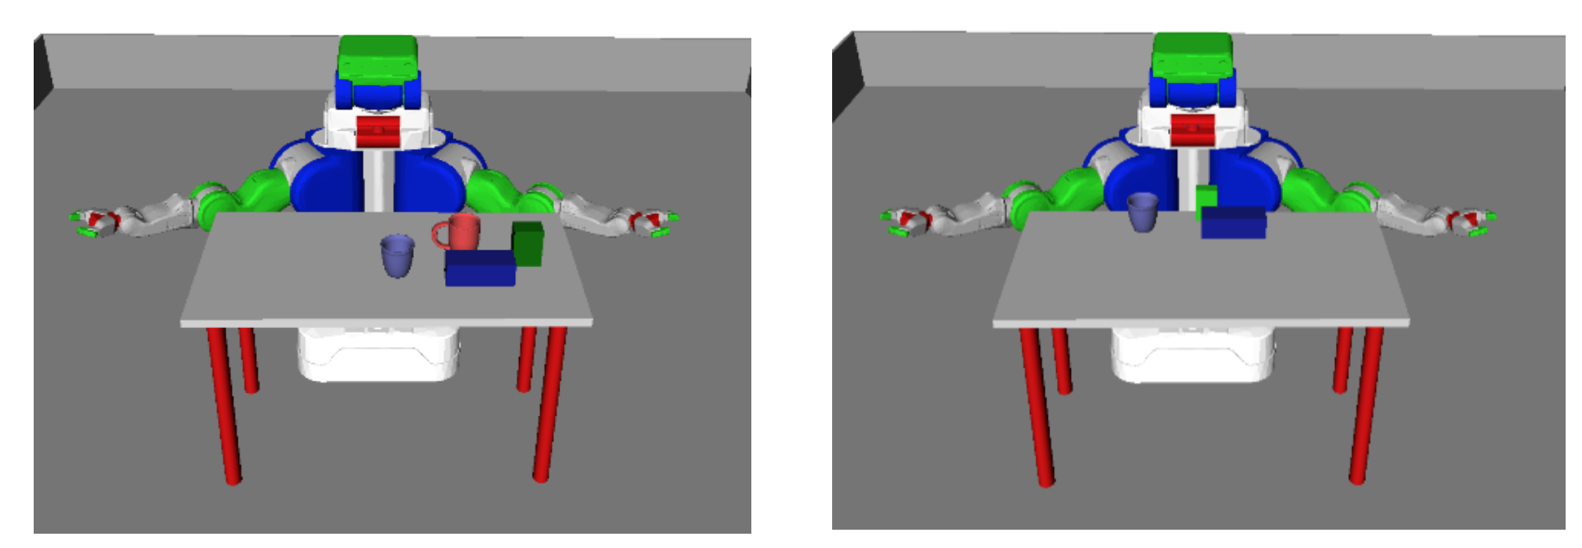
\includegraphics[scale=0.33]{./figures/choosing_grasp}
\caption{Two different instances of grasp selection domain. The robot's objective
is to plan a its left hand motion to a pregrasp pose for the blue object. The arrangement
and existence of obstacles are random across different planning
problem instances.
}
\label{fig:grasp_domain}
\end{figure}

% What is the objective fcn?
The goal for this experiment is to select a grasp 
that can be reached ``robustly'', that is, the grasp 
approach motion is collision-free under control uncertainty 
and/or uncertainty in poses of objects. 
We measure robustness as the average (over the obstacles)
of the minimum distance to each obstacle, when we plan 
a path to the selected grasp. That is,
let the plan $P_\theta := \{c_1=c_{init},c_2,\ldots,c_{n-1},c_n=c_\theta\}$, be a path
of robot's left arm and torso, which consists of a sequence
of robot configuration from initial configuration
$c_{init}$, to  the pregrasp configuration, $c_\theta$. Then, the function 
that we would like to maximize is
\begin{align*}
J^z(\theta) = \begin{cases}
\frac{\sum_{i=1}^{n} min\_dist\_to\_obs(c_i)}{n}\text{ if $\theta$ feasible}\\
-0.0719, \text{ otherwise}
\end{cases}\numberthis \label{eq:dist_fcn}\\
\end{align*}
where $\min$ operator over matrix $\mathfrak{J}$ returns the minimum element
of the matrix, and the $avg$ operator takes the average of
the elements in the matrix.  $min\_dist\_to\_obs$ function calculates the distance
to the closest obstacle from the robot at each node of the planned trajectory.

% What is the training data, and how was it generated? 
	% What is the solver?
	% What is the ScoreSolutionConstraint function?
We consider 121 different grasps, computed with OpenRAVE
grasp model function, with 479 training problem instances. 
We pass these precomputed 121 grasps as $\Theta$ to BOX.
The training data were generated by trying all the grasps
in each of 479 scenes, and recording the score of the
motion that the RRT generates. Our $ScoreSolutionConstraint$ 
function works as follows. Given grasp, 
it checks whether there exists a collision-free inverse kinematics. 
If the grasp fails to find one, then we give the grasp
a reward of zero. Otherwise, 
we call RRT to plan a motion. If RRT fails 
to find a path, then the grasp receives a reward of zero.
If it succeeds in finding a path,
then the path gets scored using the function (\ref{eq:dist_fcn}).


% What is a planning problem instnace? how is it generated?
% What's the robot's setup? DOF?
Solver for this domain is a random sampler that 
tries a grasp without replacement until a feasible one is found. Unlike
the random sampling algorithm, this one stops searching as soon as
a feasible grasp is found instead of sampling $k$ grasps. Solver 
has a time limit of 120 seconds. If it cannot find a grasp within 120 seconds,
then it receives a reward of 0.

% What is the input to the algorithm? 
The inputs to BOX were: 
$n=479,C_{1,i}=10,C_{2,i}=2, i=1,\ldots,m,\Theta=openrave\_grasps$.  
Figure \ref{fig:ff_bar_grasp} shows the comparison of algorithms
for average time for finding the first feasible plan for each problem instance.
\begin{figure}[htb]
\centering
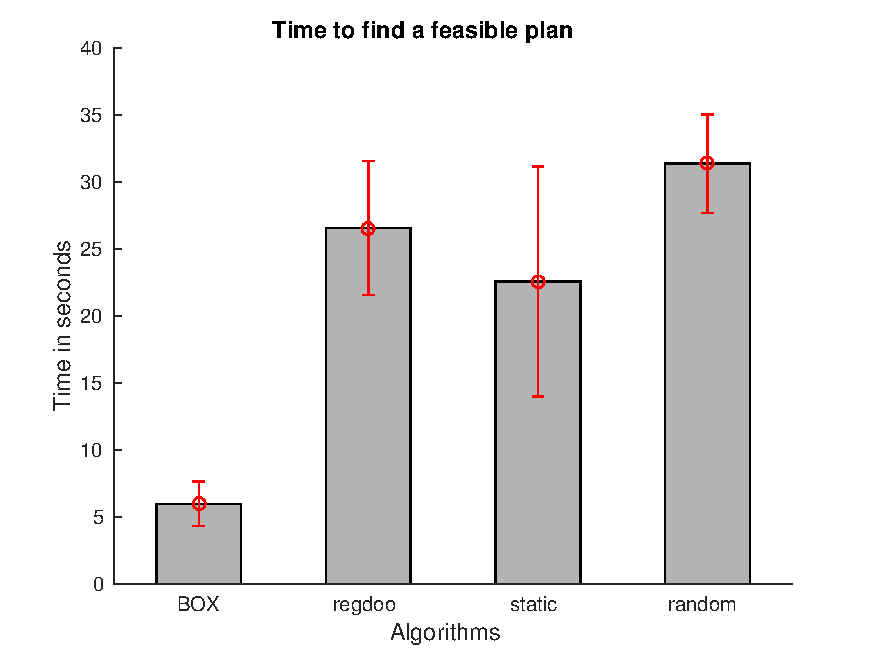
\includegraphics[scale=0.5]{./figures/only_grasp_feas_plot.pdf}
\caption{ Average time required by each algorithm over all problem instances to 
find a feasible plan with 95\% confidence interval.}
\label{fig:ff_bar_grasp}
\end{figure} 
Solver, which randomly samples a grasp without replacement, takes
close to 6 times that of the BOX. RegDOO and static algorithms
are much more slower than BOX, each requiring multiple factor 
of the time required by BOX.


\begin{figure}[htb]
\centering
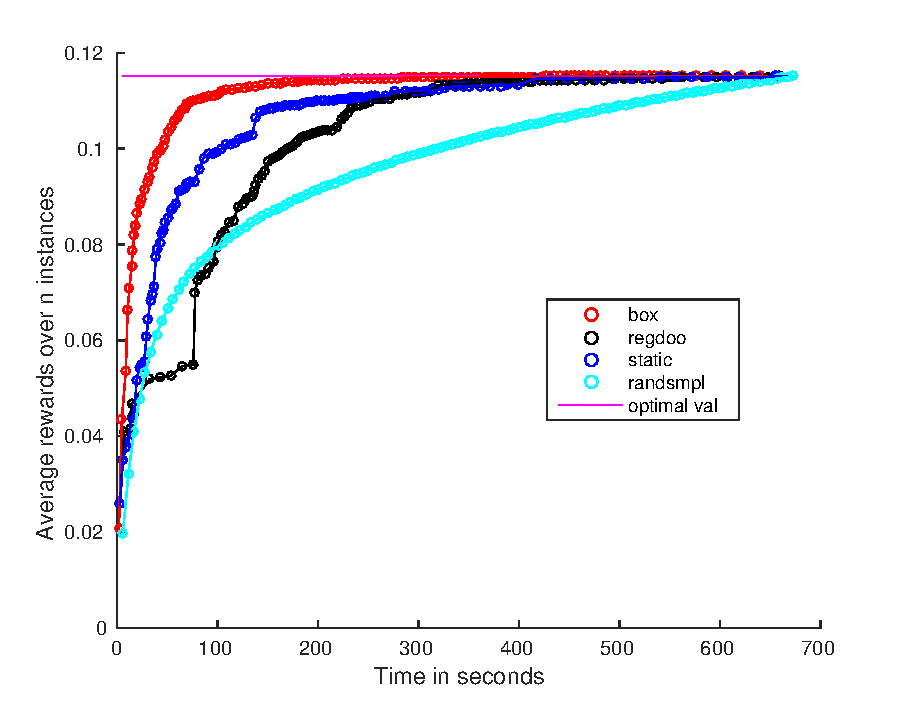
\includegraphics[scale=0.5]{./figures/only_grasp_vs_t.pdf}
\caption{ Grasp domain }
\label{fig:only_grasp_t}
\end{figure} 


\iffalse
Figure \ref{fig:time_limit_scores_grasp} shows, given the same
or multiples of amount of time required by the solver to find
 the first feasible plan, how much improvement in score 
can each algorithm provide.
\begin{figure}[htb]
\centering
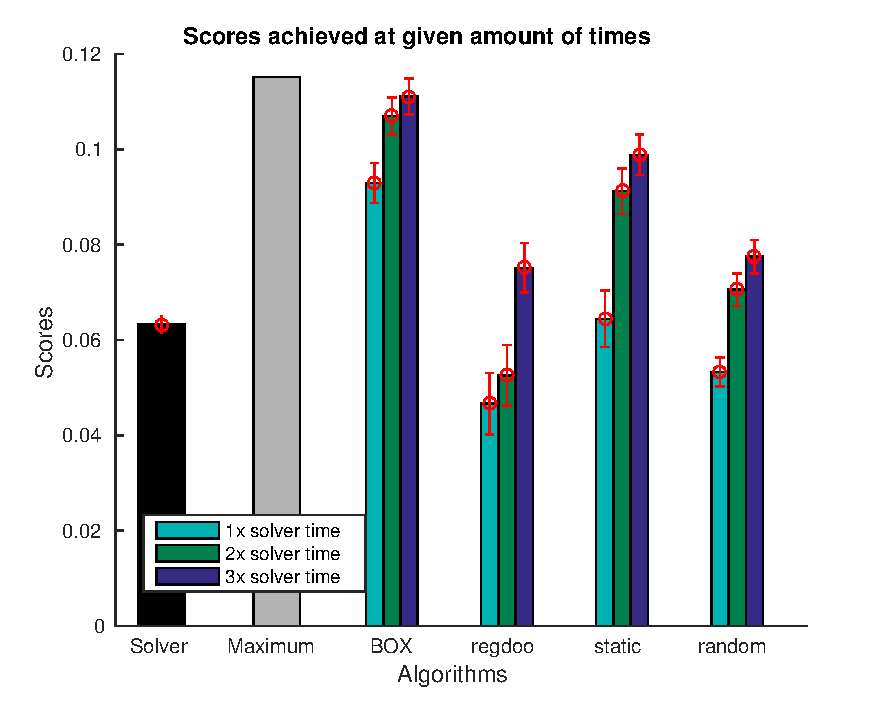
\includegraphics[scale=0.5]{./figures/only_grasp_opt_plot.pdf}
\caption{ Average score of each algorithm over all the problem instances when given 1x, 2x and 3x of amount of time for solver to find a feasible solution with 95\% confidence
interval. }
\label{fig:time_limit_scores_grasp}
\end{figure} 
As the plot shows, BOX outperformed all the other algorithms by
multiple factors. Especially, given 2x the solver time, it outperformed
all the other algorithms given 3x the solver time. 

Figure \ref{fig:time_reqd_for_opt_grasp} shows the average time required
by each algorithm to find the optimal $\theta$ for each problem instance. 
\begin{figure}[htb]
\centering
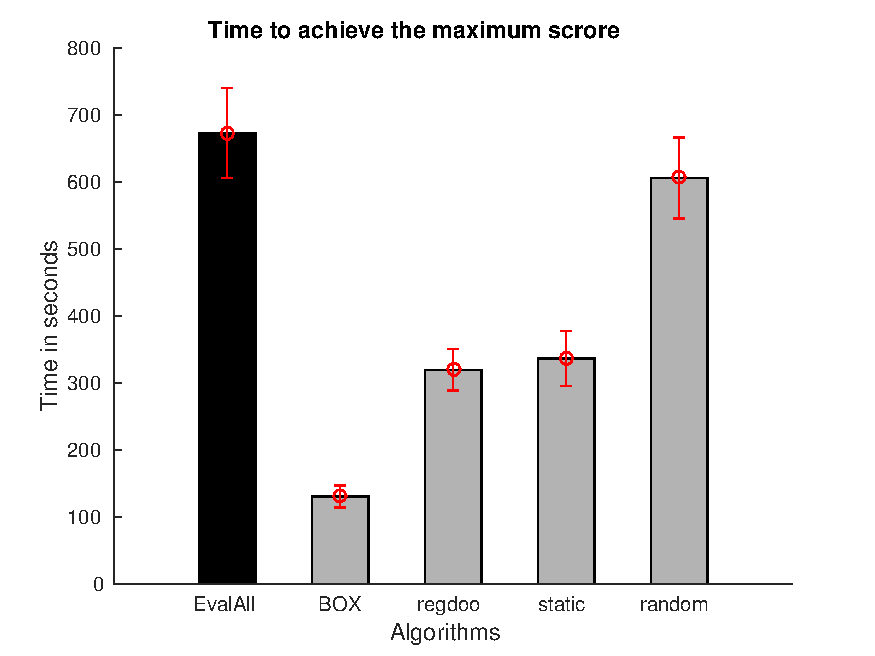
\includegraphics[scale=0.5]{./figures/only_grasp_opt_time_plot.pdf}
\caption{ Average time required by each algorithm over all the problem instances to find the best plan with 95\% confidence interval. }
\label{fig:time_reqd_for_opt_grasp}
\end{figure} 
Again, BOX outperformed all the other algorithms, requiring orders
of magnitudes less time than them. 
\fi


\subsection{Grasp and base location selection for robust motion planning}
% general description of the task
	% define the task, and what SG represent
We again tackle the robust motion planning problem in a more challenging domain.
In this experiment, the robot again needs to plan its left arm and torso
to reach a pregrasp pose, but it also needs to place its base location appropriately 
in addition to choosing a grasp in order to maximize the distances to obstacles. 
Therefore, our a solution constraint for this domain consists of the 
robot base pose, $(x,y,\psi)$,  where $\psi$ is an orientation of the robot, 
as well as one of 121 grasps.  The objective function we would like to
maximize is same as eqn. (\ref{eq:dist_fcn})


\begin{figure*}[htb]
\centering
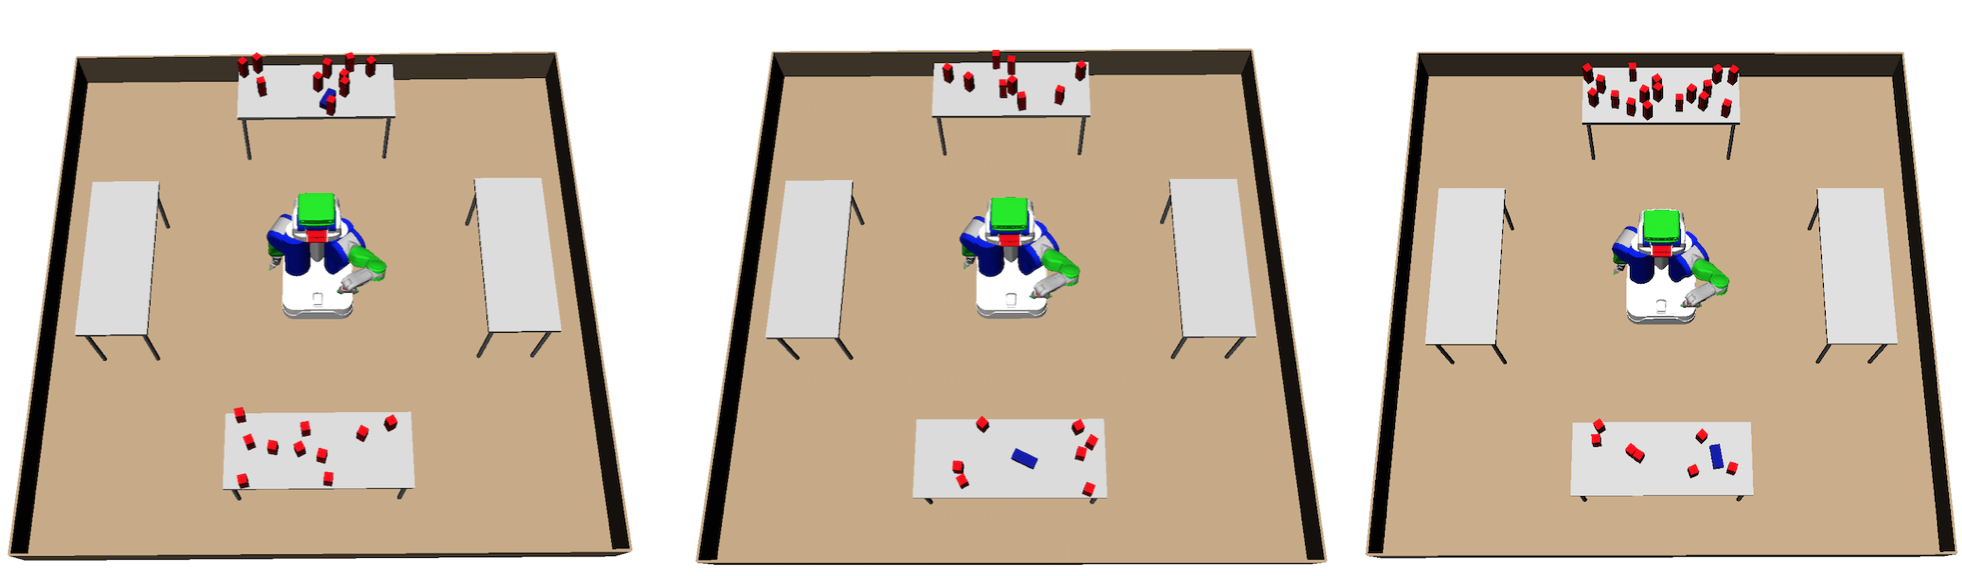
\includegraphics[scale=0.5]{./figures/choosing_base_loc_and_grasp}
\caption{Three different instances of base and grasp selection domain, with
robot at its default location. The robot needs to choose its base pose
and a grasp to plan a motion to a pregrasp configuration for the blue object. 
The poses of obstacles and the blue object is random.
}
\label{fig:gb_domain}
\end{figure*}

% What is a planning problem instnace? how is it generated?
% What's the robot's setup? DOF?
A planning problem instance is again defined by the arrangement of objects.
Figure \ref{fig:gb_domain} shows three different training scenes.
We have 20 rectangular boxes as obstacles, all standing up on the two tables.
The $(x,y)$ location and orientation about $z-axis$ of each of the obstacles 
are randomly chosen.
The object to be picked up, colored in blue, is lying on either one of the
two tables at random, with random orietntation about $z-axis$ and $(x,y)$. 
The robot always starts at the same base pose, with same arm configuration.
The robot has 3 active DOFs when it is required to move its base to a
pick-up base pose. Once it gets there,
the robot then has 8 active DOFs, including its left arm and torso. We omit
the base motion planning and only consider arm motion for evaluation.

% What is the training data, and how was it generated? 
	% What is the solver?
	% What is the ScoreSolutionConstraint function?
Given a planning problem instance, Solver for this domain performs 
three procedures. First, it randomly samples a base pose, $(x,y,\psi)$,  
from a continuous, reachable and collision free region of the space. It then
tests 121 grasps sequentially until a collision free inverse 
kinematics is found. Lastly, it calls RRT at this base pose, to the
collision free pregrasp configuration, and see checks if the path exists.
If there is, then  this pair of the chosen grasp $g$ and 
the robot pose $(x,y,\psi)$ becomes a solution constraint, and is added to our library.
Once we have constructed the library, for each problem instance and a constraint,
$ScoreSolutionConstraint$ function then calls RRT
using the constraint, and then score them according to eqn. (\ref{eq:dist_fcn}), with the
score of -0.3927 for the infeasible constraints.
However, if the base pose is in collision, or if a reachable collision-free pick-up 
base location is found but none of the grasps have collision-free inverse kinematics, 
or RRT fails to find a path, the constraint is assigned a score of 0. 

% What is the input to the algorithm? 
The inputs to BOX were 
$n=988,u=1,C_{1,i}=10,C_{2,i}=1, i=1,\ldots,m, \Theta=\{\}$.  We then
 discarded some of the generated solution constraints and reduced the
 $|\Theta|=486$, to speed up the training data generation. 
\footnote{This step is completely unnecessary if time for training data
 generation is not of a concern}. Figure \ref{fig:ff_bar_pick_base} 
shows the average time for algorithms to generate the first feasible plan.
\begin{figure}[htb]
\centering
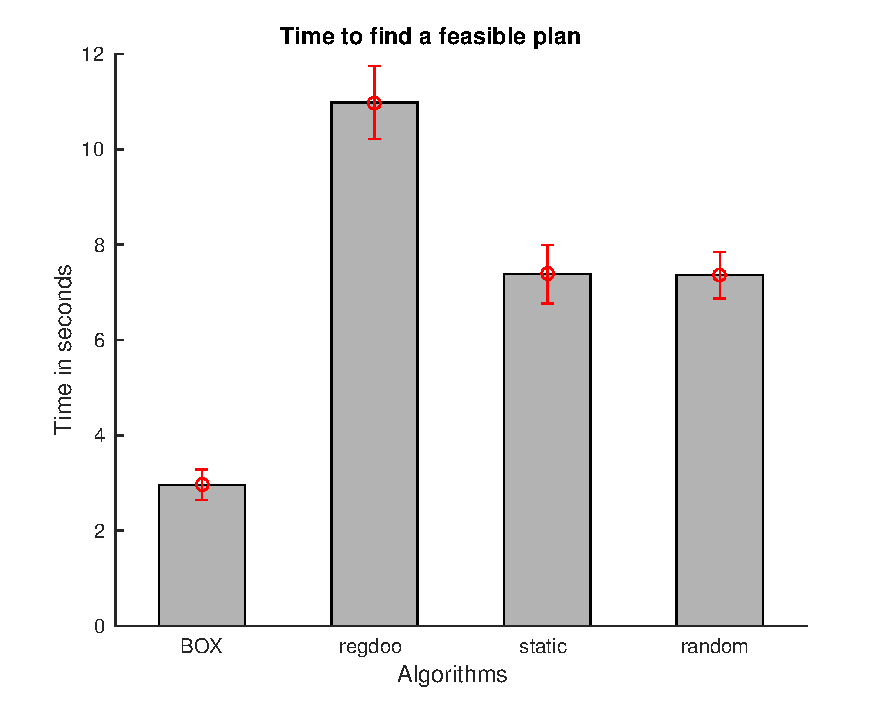
\includegraphics[scale=0.5]{./figures/pick-place_feas_plot.pdf}
\caption{ Average time required by each algorithm to find a feasible plan for a problem instance.}
\label{fig:ff_bar_pick_base}
\end{figure} 
Unlike the previous domain, the library-based algorithms completely
outperformed Solver. This is because compared to computing the
inverse kinematics from sampled grasp and base pose and planning 
the left arm motion, sampling a feasible $\theta$ takes 
significantly more time. Out of all the library based methods,
 BOX again outperformed all the other
algorithms by multiple factors.

\begin{figure}[htb]
\centering
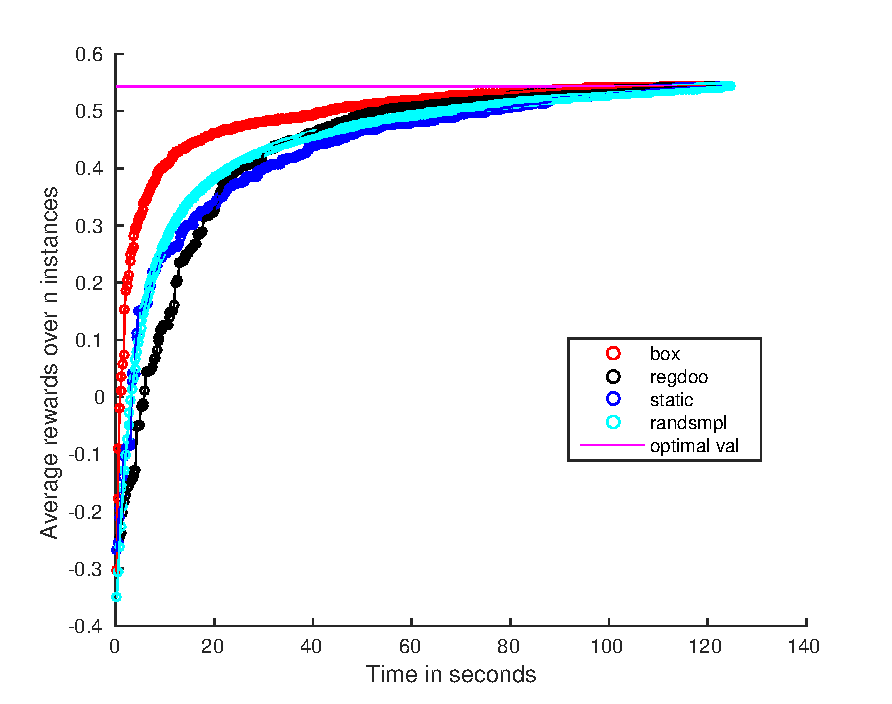
\includegraphics[scale=0.5]{./figures/pick-place_vs_t.pdf}
\caption{ pick-base domain.}
\label{fig:pick-base_vs_t}
\end{figure} 

\iffalse

Figure \ref{fig:time_limit_scores_grasp} shows the improvement in scores
over solver when given the 1/10,2/10 , and 3/10 of the time
 required by the solver to find the first feasible plan.
\begin{figure}[htb]
\centering
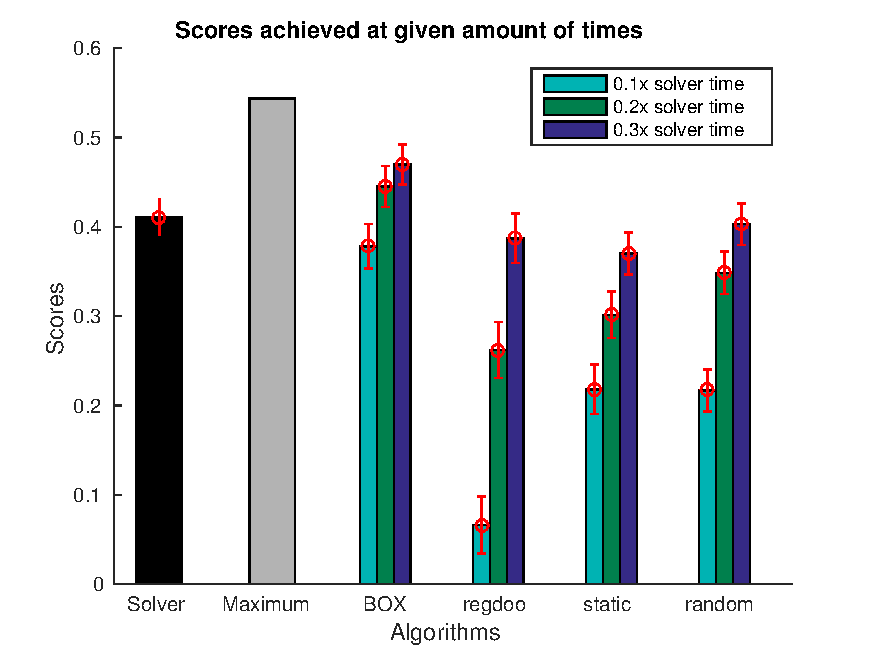
\includegraphics[scale=0.5]{./figures/pick-place_opt_plot.pdf}
\caption{ Average score of each algorithm when given 0.1x, 0.2x and 0.3x of the time required by Solver to find a feasible solution. }
\label{fig:opt_plot_pick_base}
\end{figure} 
Given 1/10 of the time, no algorithm can provide a better quality
plan than Solver. However, with 2/10 and 3/10 
of the time, BOX is ale to provide improvement over Solver, compared
to other algorithms who cannot.

Figure \ref{fig:opt_time_plot_pick_base} shows the average time required by each
algorithm to find the optimal $\theta$ for each problem instance.
\begin{figure}[htb]
\centering
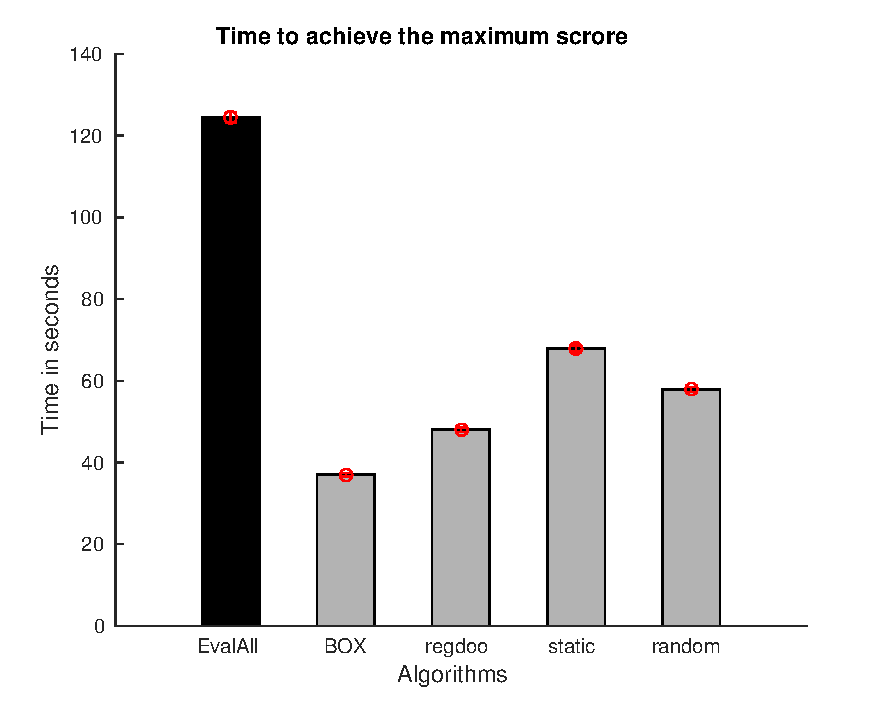
\includegraphics[scale=0.5]{./figures/pick-place_opt_time_plot.pdf}
\caption{Average time required by each algorithm to find the best plan for each problem instance. }
\label{fig:opt_time_plot_pick_base}
\end{figure} 
BOX again was the fastest algorithm to find the optimal $\theta$.
\fi


\subsection{Grasp, base location, object placement pose, 
	    and partial path selection for shortest path planning
	    with varying robot shape
		}
% general description of the task
	% define the task, and what SG represent
In this experiment, the robot needs to pick-and-place an object
from one table to another, where there is a narrow passage
in between, using its left arm, torso, and base motions. 
To do this, the robot first needs to choose three variables:
a grasp, $g$, an object placement pose, $p_{obj}$, which consists of 
$(x,y)$ location on the other table and its orientation
about the $x-axis$, a robot base pose, $p_{robot}$, for placing the
object at $p_{obj}$. Once the robot chooses these variables,
it calls RRT to generate three paths: the pregrasp
configuration, a path from the initial base pose to $p_{robot}$,
and then a path for placing the object at $p_{obj}$. In addition
to forementioned three variables, we would like to suggest
subgoals for each of these paths. Therefore, a solution 
constraint in this domain would consists of six variables,
$[g,p_{obj},p_{robot},sg_{pregrasp},sg_{base},sg_{place}]$,
where $sg$ denotes the subgoal for each path.
The objective here is to minimize the total distance
travelled by the robot's leftarm, torso, and base.

% What is a planning problem instnace? how is it generated?
% What's the robot's setup? DOF?
Unlike the previous two experiments where a problem
instance was defined only by arrangements of obstacles,
here a problem instance is defined by both the obstacle arrangement
and the length of the object to be transported. 
We have in total 28 rectangular obstacles, all standing up, whose 
$(x,y)$ locations on either table is chosen randomly. The 
initial pose of the object to be transported remains the same across
different problem instances, while 
its length is chosen randomly from three different values.
Figure \ref{fig:biggest_domain}  shows three different training scenes. 
Here, when the robot is holding the black object with different lengths,
this effectively changes the shape of the robot, and it needs
 different maneuvers
to get through the passage for different shapes. More specifically,
since the longest rod has length greater than the width of
the passage, the robot needs to turn its base in order to get
through it. The robot has 
8 active DOFs for planning its left arm and torso motions 
for pregrasp and placing,
and 3 active DOFs for planning its base pose to $p_{robot}$.

\begin{figure}[htb]
\centering
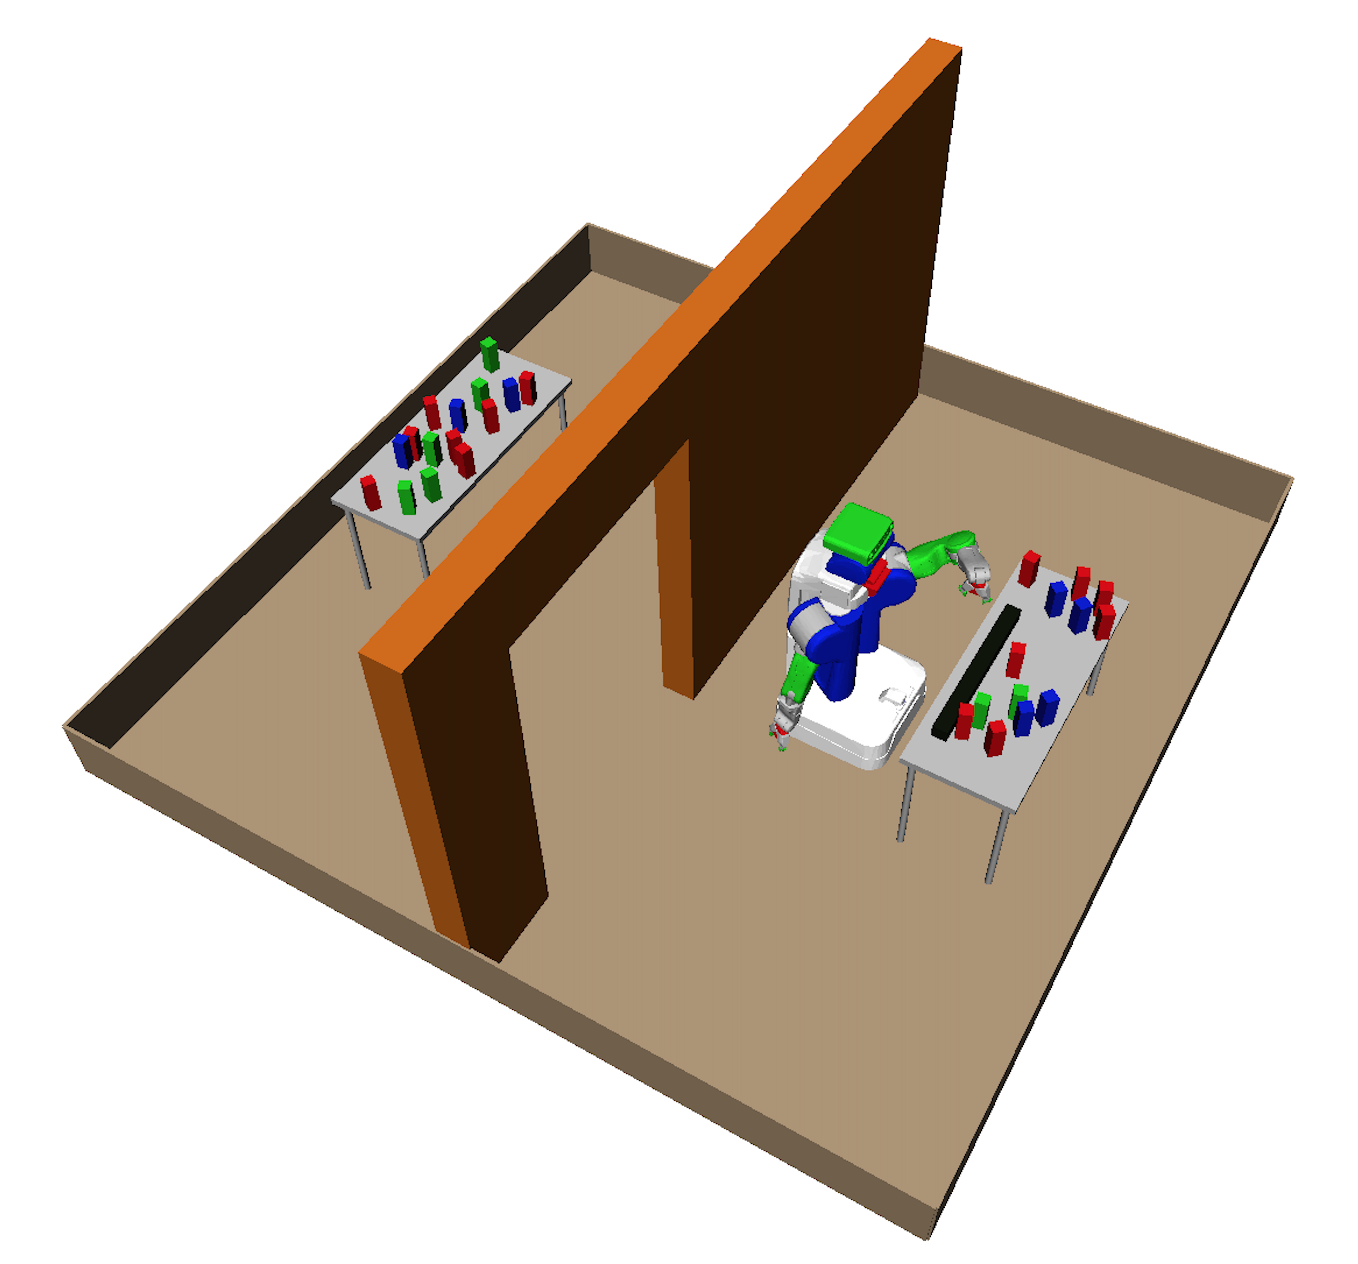
\includegraphics[scale=0.18]{./figures/biggest1}
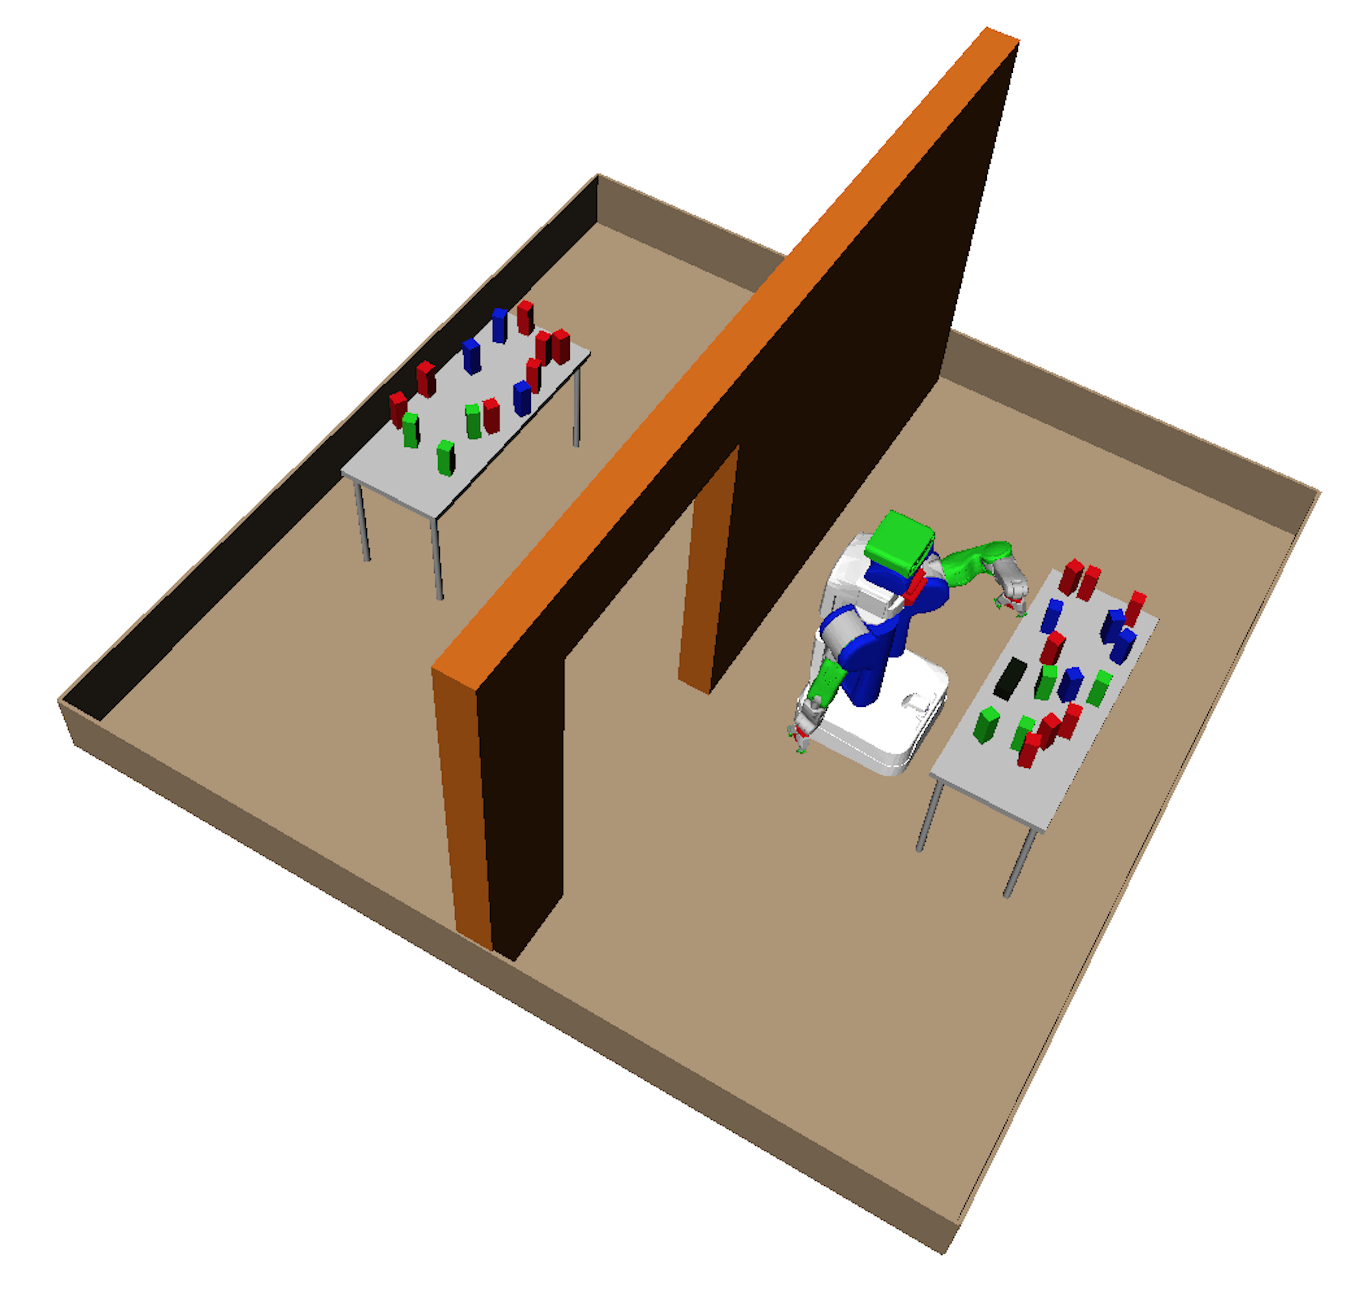
\includegraphics[scale=0.18]{./figures/biggest2}
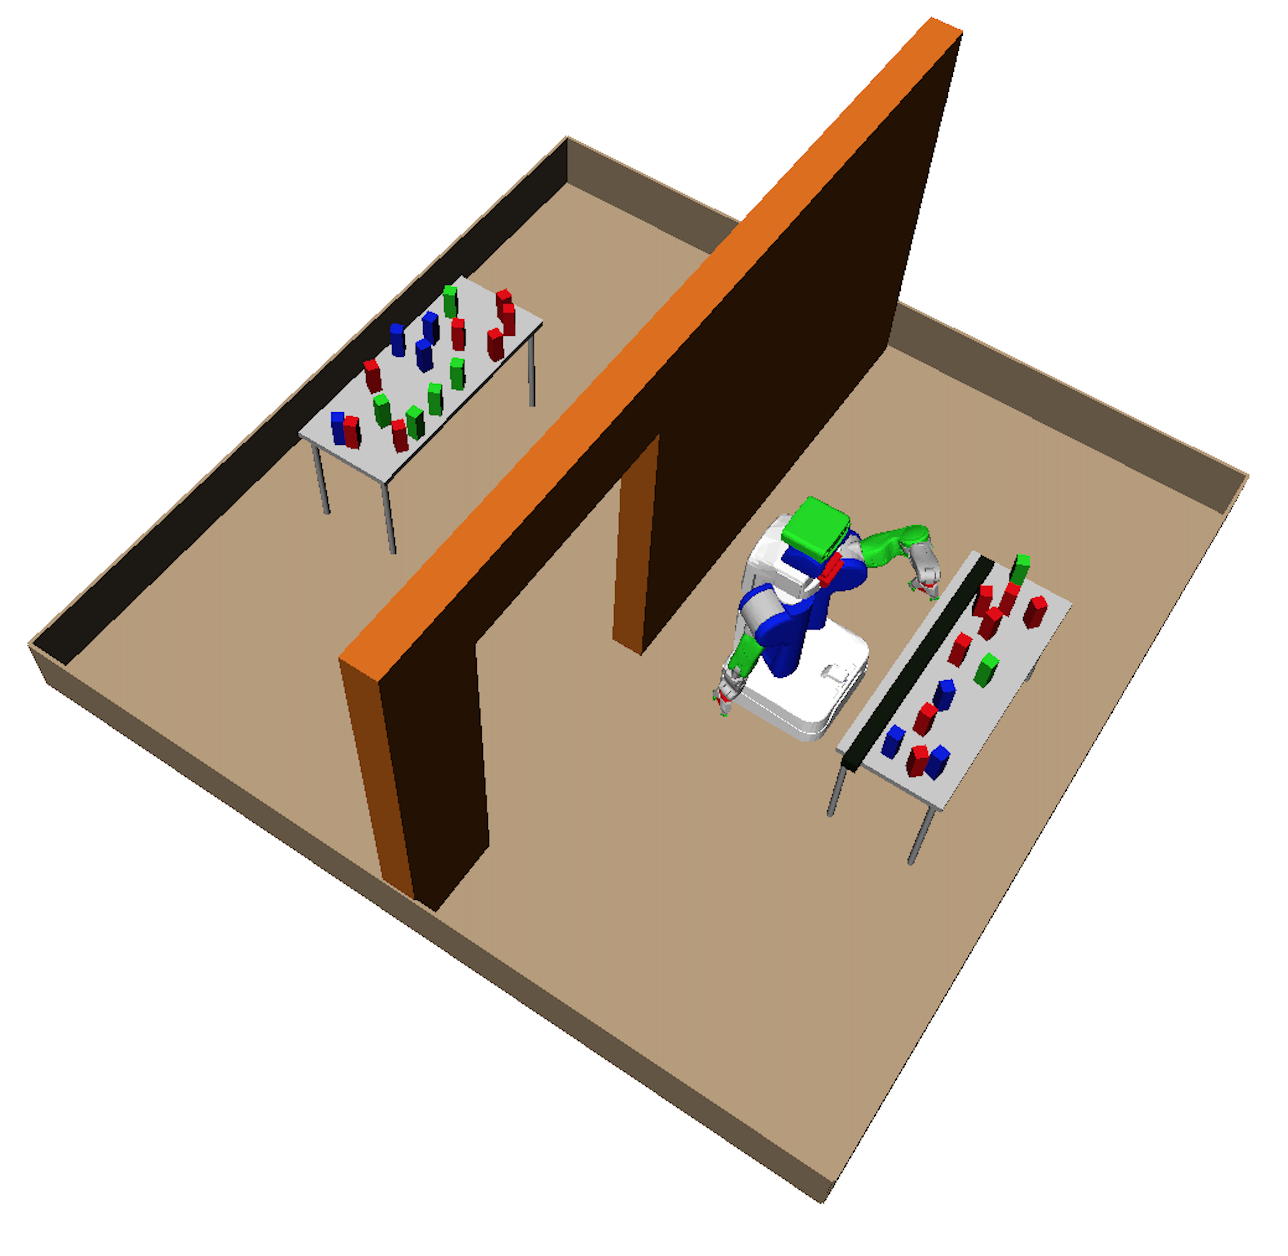
\includegraphics[scale=0.18]{./figures/biggest3}
\caption{Three different instances of the pick-and-place domain.
The robot needs to transport the black object, whose length is
randomly chosen from the three lengths shown, to the other table. The obstacle arrangements
across different scenes are random as well. The initial pose of
the black object is the same across all planning problem instances.}
\label{fig:biggest_domain}
\end{figure}


% What is the training data, and how was it generated? 
	% What is the solver?
Given a planning problem instance, Solver first randomly
samples $g,p_{obj},p_{robot}$ by first finding the
feasible grasp, then choosing the $p_{obj}$ for which
inverse kinematics yields the $g$. Then, it samples
collision free $p_{robot}$ for which this grasp is
reachable. Once it finds chose these variables,
it, then it calls RRT
for computing three different paths: a pickup motion,
a base motion, and a place motion. To construct
a library, we then choose, as our subgoals for these paths, the 
configuration that minimizes the distance
travelled by the robot when planned from the initial
configuration to the subgoal then to the goal pose. If all
these are feasible, we then add it to the library,
otherwise discard it.

% What is the objective fcn?
Once we have constructed the library, for each
problem instance and a constraint, $ScoreSolutionConstraint$
function calls RRT with the constraint and score
the computed motion with the function
\begin{align*}
J^z(\theta) = \begin{cases}
		-length(P_\theta), \text{ if $\theta$ feasible}\\
		\min(\mathfrak{J})-|avg(\mathfrak{J})|, \text{ otherwise}
	      \end{cases} \numberthis \label{eq:minlen_fcn}
\end{align*}
where $\min$ operator over matrix $\mathfrak{J}$ returns the minimum element
of the matrix, and the $avg$ operator takes the average of
the elements in the matrix.

% What is the input to the algorithm? 
The inputs to BOX were: $n=600, u=1, C_1=10, C_2=2 $, and we discarded 
some of $\theta$ so that $|\Theta| = 586$.
Figure \ref{fig:ff_bar_pp} shows the average time for finding the first feasible
plan. This domain again required Solver to sample a value from
continuous domain, such as $p_{obj}$ and $p_{robot}$, which gave
the library-based approaches more advantage. Moreover, the narrow
passage made the plain RRT, without subgoal, to have more planning
time than those with subgoal. These two advantages allowed the library
based algorithms to compute a plan faster, with BOX as fastest algorithm, 
with more than 4 times faster than Solver. Static
came next, which was more than 2 times faster than Solver. Random sampler
struggled the most, with its speed almost same as Solver.

\begin{figure}[htb]
\centering
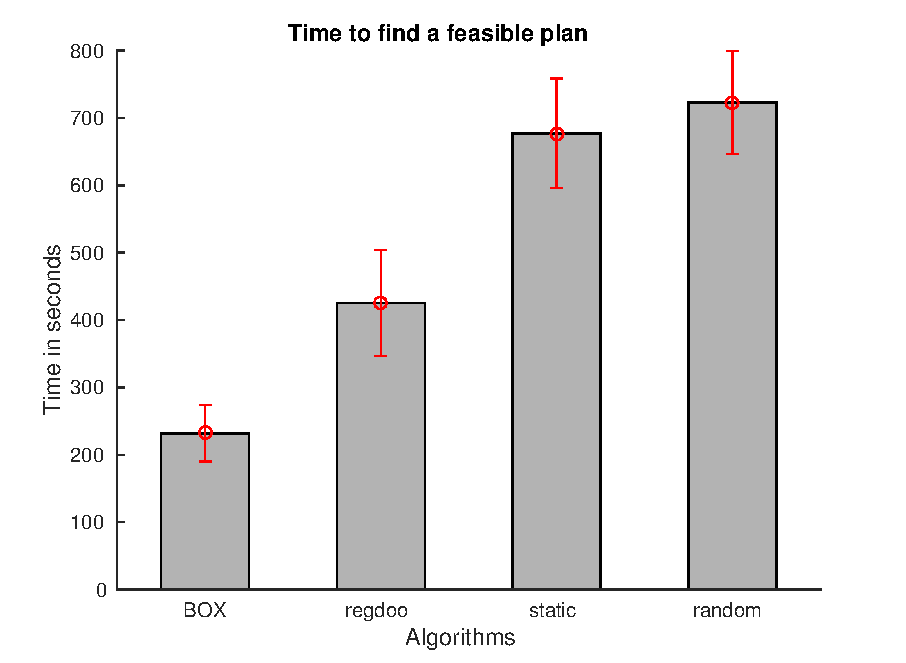
\includegraphics[scale=0.5]{./figures/place_and_partial_path_feas_plot.pdf}
\caption{ Average time required by each algorithm to find a feasible plan for each problem instance.}
\label{fig:ff_bar_pp}
\end{figure} 

\begin{figure}[htb]
\centering
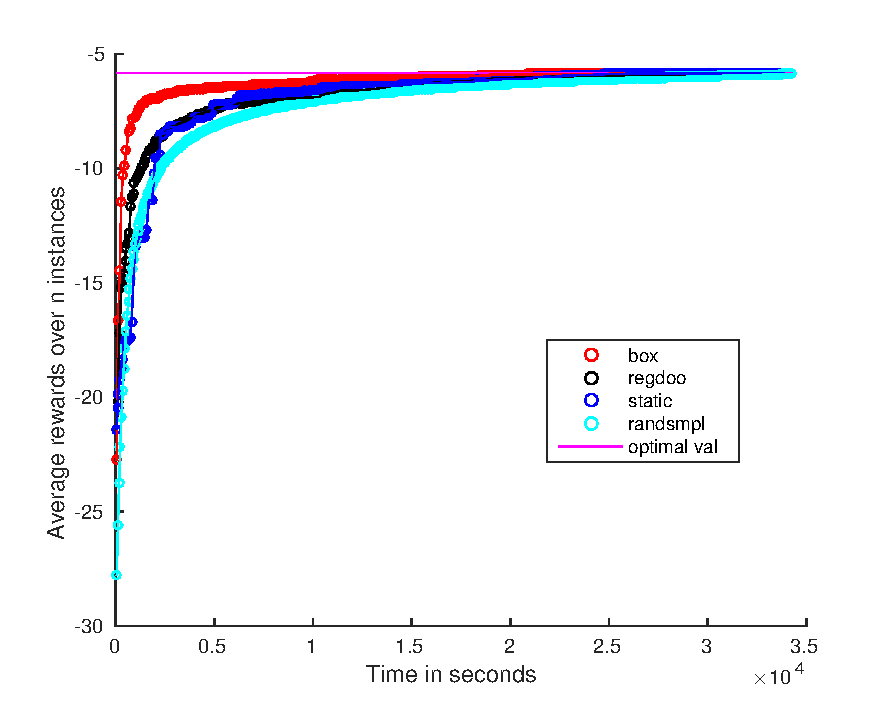
\includegraphics[scale=0.5]{./figures/place_and_partial_path_vs_t.pdf}
\caption{ Biggest domain.}
\label{fig:biggest_vs_t}
\end{figure} 

\iffalse
Figure \ref{fig:opt_plot_pp} shows the average scores of algorithms when
given different amount of time limits. Given the same amount of
time as Solver, BOX was able to produce the best quality plan compared
to all the other algorithms. Especially, it performed almost
twice better than Solver. For 2x and 3x time required by the solver,
BOX was able to provide the best quality plan among algorithms as well.
One observation from this plot is that, in all the algorithms,
 there is a very small improvement from 2x to 3x. This is due to
the fact that, in problem instances with the longest black object,
a call to RRT takes significant amount of time. Hence making improvements,
which requires more evaluations, is more costly than the previous two
domains. 


\begin{figure}[htb]
\centering
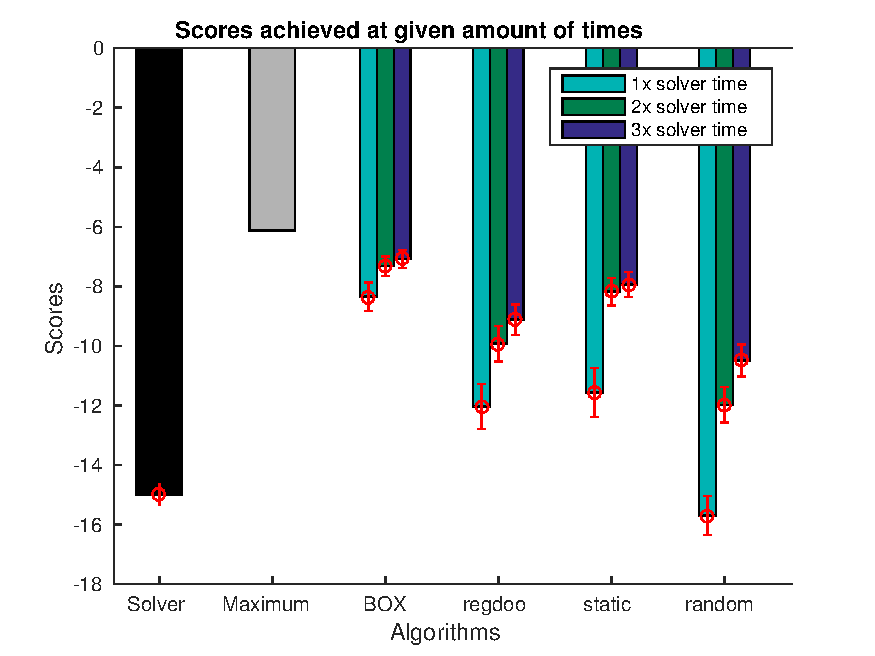
\includegraphics[scale=0.5]{./figures/place_and_partial_path_opt_plot.pdf}
\caption{ Average score of each algorithm when given the 1x, 2x and 3x of time required by solver to find a feasible solution. }
\label{fig:opt_plot_pp}
\end{figure} 

Figure \ref{fig:opt_time_plot_pp} shows the time required by each algorithm
to find the optimal $\theta$. Again, BOX outperformed all the other algorithms
by multiple factors. We can see the effect of longer-stick problem instances
in here as well. The solver, which finds the first feasible solution and
then quits, took on average about 850 seconds. BOX on the other hand,
which tries to find the best $\theta$ for each scene, requires more evaluations
than Solver. This caused the computation time to be near 5000 seconds, which
is close to 6 times than that of the solver, for the improvement in plan quality
by factor of around 2.5.


\begin{figure}[htb]
\centering
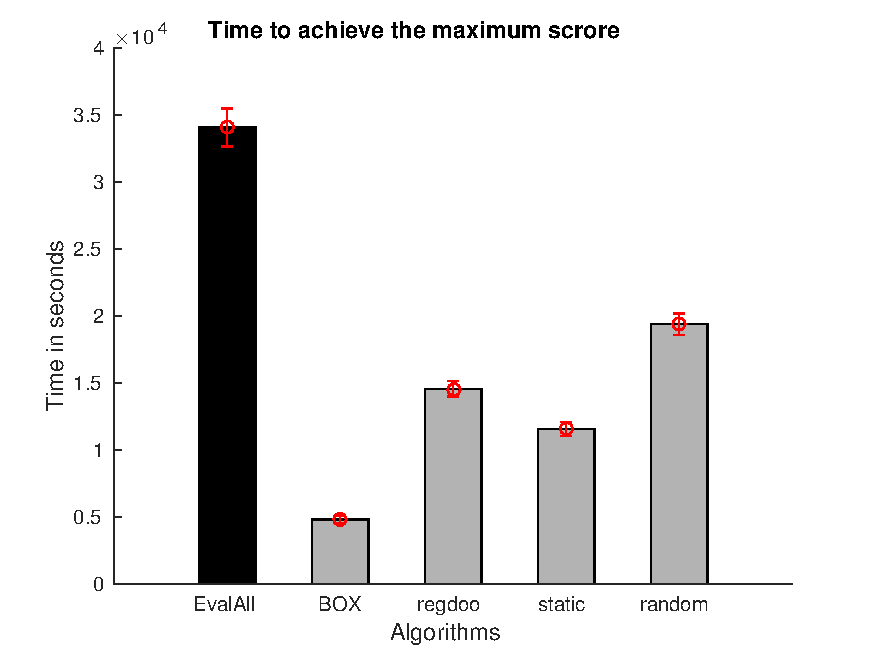
\includegraphics[scale=0.5]{./figures/place_and_partial_path_opt_time_plot.pdf}
\caption{ Average time required by each algorithm to find the best plan for each problem instance. }
\label{fig:opt_time_plot_pp}
\end{figure} 
Figure \ref{fig:opt_plot_pp} shows the average scores of algorithms when
given different amount of time limits. Given the same amount of
time as Solver, BOX was able to produce the best quality plan compared
to all the other algorithms. Especially, it performed almost
twice better than Solver. For 2x and 3x time required by the solver,
BOX was able to provide the best quality plan among algorithms as well.
One observation from this plot is that, in all the algorithms,
 there is a very small improvement from 2x to 3x. This is due to
the fact that, in problem instances with the longest black object,
a call to RRT takes significant amount of time. Hence making improvements,
which requires more evaluations, is more costly than the previous two
domains. 


\begin{figure}[htb]
\centering
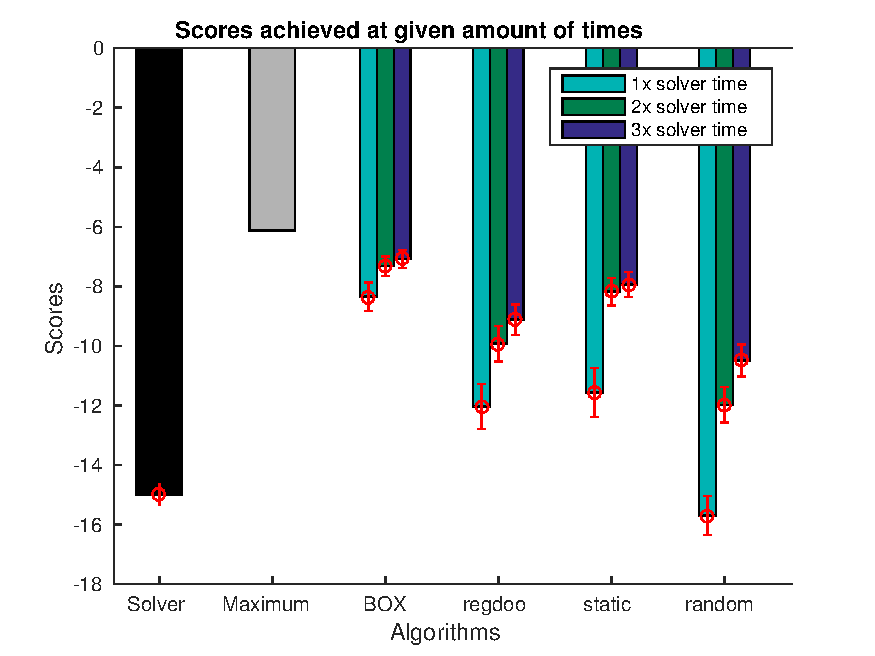
\includegraphics[scale=0.5]{./figures/place_and_partial_path_opt_plot.pdf}
\caption{ Average score of each algorithm when given the 1x, 2x and 3x of time required by solver to find a feasible solution. }
\label{fig:opt_plot_pp}
\end{figure} 

Figure \ref{fig:opt_time_plot_pp} shows the time required by each algorithm
to find the optimal $\theta$. Again, BOX outperformed all the other algorithms
by multiple factors. We can see the effect of longer-stick problem instances
in here as well. The solver, which finds the first feasible solution and
then quits, took on average about 850 seconds. BOX on the other hand,
which tries to find the best $\theta$ for each scene, requires more evaluations
than Solver. This caused the computation time to be near 5000 seconds, which
is close to 6 times than that of the solver, for the improvement in plan quality
by factor of around 2.5.


\begin{figure}[htb]
\centering
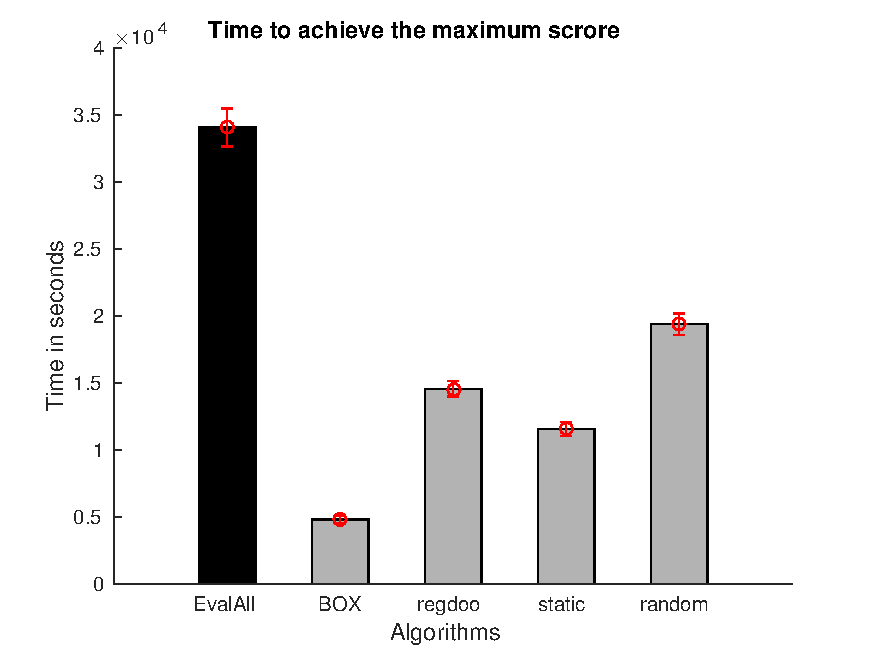
\includegraphics[scale=0.5]{./figures/place_and_partial_path_opt_time_plot.pdf}
\caption{ Average time required by each algorithm to find the best plan for each problem instance. }
\label{fig:opt_time_plot_pp}
\end{figure} 
\fi
